\documentclass[a4paper]{article} 

\usepackage{listings}
\usepackage{xcolor}
\definecolor{codegreen}{rgb}{0,0.6,0}
\definecolor{codegray}{rgb}{0.5,0.5,0.5}
\definecolor{codeorange}{rgb}{1,0.49,0}
\definecolor{backcolour}{rgb}{0.95,0.95,0.96}

\lstdefinestyle{mystyle}{
    backgroundcolor=\color{backcolour},   
    commentstyle=\color{codegray},
    keywordstyle=\color{codeorange},
    numberstyle=\tiny\color{codegray},
    stringstyle=\color{codegreen},
    basicstyle=\ttfamily\footnotesize,
    breakatwhitespace=false,         
    breaklines=true,                 
    captionpos=b,                    
    keepspaces=true,                 
    numbers=left,                    
    numbersep=5pt,                  
    showspaces=false,                
    showstringspaces=false,
    showtabs=false,                  
    tabsize=2,
    xleftmargin=10pt,
}

\lstset{style=mystyle}

\addtolength{\hoffset}{-2.25cm}
\addtolength{\textwidth}{4.5cm}
\addtolength{\voffset}{-3.25cm}
\addtolength{\textheight}{5cm}
\setlength{\parskip}{0pt}
\setlength{\parindent}{0in}

%----------------------------------------------------------------------------------------
%	PACKAGES AND OTHER DOCUMENT CONFIGURATIONS
%----------------------------------------------------------------------------------------

\usepackage{blindtext} % Package to generate dummy text
\usepackage{charter} % Use the Charter font
\usepackage[utf8]{inputenc} % Use UTF-8 encoding
\usepackage{microtype} % Slightly tweak font spacing for aesthetics
\usepackage[english]{babel} % Language hyphenation and typographical rules
\usepackage{amsthm, amsmath, amssymb} % Mathematical typesetting
\usepackage{float} % Improved interface for floating objects
\usepackage[final, colorlinks = true, 
            linkcolor = black, 
            citecolor = black]{hyperref} % For hyperlinks in the PDF
\usepackage{graphicx, multicol} % Enhanced support for graphics
\usepackage{xcolor} % Driver-independent color extensions
\usepackage{marvosym, wasysym} % More symbols
\usepackage{rotating} % Rotation tools
\usepackage{censor} % Facilities for controlling restricted text
\usepackage{listings, style/lstlisting} % Environment for non-formatted code, !uses style file!
\usepackage{pseudocode} % Environment for specifying algorithms in a natural way
\usepackage{style/avm} % Environment for f-structures, !uses style file!
\usepackage{booktabs} % Enhances quality of tables
\usepackage{tikz-qtree} % Easy tree drawing tool
\tikzset{every tree node/.style={align=center,anchor=north},
         level distance=2cm} % Configuration for q-trees
\usepackage{style/btree} % Configuration for b-trees and b+-trees, !uses style file!
\usepackage{csquotes} % Context sensitive quotation facilities
\usepackage[yyyymmdd]{datetime} % Uses YEAR-MONTH-DAY format for dates
\renewcommand{\dateseparator}{-} % Sets dateseparator to '-'
\usepackage{fancyhdr} % Headers and footers
\pagestyle{fancy} % All pages have headers and footers
\fancyhead{}\renewcommand{\headrulewidth}{0pt} % Blank out the default header
\fancyfoot[L]{} % Custom footer text
\fancyfoot[C]{} % Custom footer text
\fancyfoot[R]{\thepage} % Custom footer text
\newcommand{\note}[1]{\marginpar{\scriptsize \textcolor{red}{#1}}} % Enables comments in red on margin

%----------------------------------------------------------------------------------------

\begin{document}

%-------------------------------
%	TITLE SECTION
%-------------------------------

\fancyhead[C]{}
\hrule \medskip % Upper rule
\begin{minipage}{0.295\textwidth} 
    \begin{raggedright}
        \footnotesize
        Andrew Hayes \hfill\\   
        21321503 \hfill\\
        a.hayes18@nuigalway.ie 
    \end{raggedright}
\end{minipage}
\begin{minipage}{0.4\textwidth} 
    \begin{centering}
        \large 
        CT2109 Assignment 2\\ 
        \normalsize 
    \end{centering}
\end{minipage}
\begin{minipage}{0.295\textwidth} 
    \begin{raggedleft}
        \footnotesize
        \today \hfill\\
    \end{raggedleft}
\end{minipage}

\medskip\hrule 
\medskip
\begin{centering}
    Solving Expressions in Postfix Notation Using Stacks\\ 
\end{centering}
\medskip\hrule 
\bigskip

\section{Problem Statement}
The problem here is a reasonably basic one. 
We want to create a program that allows a user to enter an arithmetic expression in conventional algebraic form (infix 
notation), calculates the answer to the expression using a Stack, and displays the results to the user. 
The precedence rules outlined in the assignment specification are the well-known BIMDAS (sometimes PEMDAS), meaning that 
Brackets have the highest precedence, followed by Indices, followed by Multiplication \& Division, followed by Addition 
\& Subtraction.
\\\\
To use a Stack to perform the calculations, the expression must first be converted from infix notation to postfix notation. 
This allows a much simpler way of evaluating the expressions. 
If infix was used on the stack, with one symbol per ``slot'' or index in the stack, the symbol at the top of the stack would 
be an operand. 
Our program would need to pop the stack several times before it could determine what it was actually supposed to do with said
operand. 
If postfix notation was used, our program knows exactly what to do because the first symbol on the stack will be an operator. 
When an operator is encountered, the program will know that the operator requires two operands and pop them from the stack, 
avoiding any amount of guesswork or confusion that infix notation would've caused.

\section{Analysis \& Design Notes}
Firstly, we want to scan in the expression from the user using a \verb|Scanner| object and a \verb|String|. 
There are some rules about valid \& invalid expressions, and if the expression is invalid, we want to prompt the user to re-enter 
their expression. 
The criteria for validity are as follows: the expression must be between 3 \& 20 characters, and it must only contain single 
digits 1-9 and the symbols \verb|^|, \verb|*|, \verb|/|, \verb|+|, \verb|-|, \verb|(|, \& \verb|)|.  
In a do-while loop, we'll prompt the user to enter an expression and scan it in. 
The expression will first be checked to ensure that it is of the appropriate length. 
If not, the loop will repeat. 
If the expression is of the appropriate length, it will then be checked using a regular expression to see if it contains any 
characters that are not the allowed characters.
If so, the loop will repeat. 
If the expression does not contain any illegal characters, it will finally be checked using a regular expression to see if it 
contains numbers that have two or more digits (essentially just checking if a digit is ever followed by another digit). 
If so, the loop will repeat. 
Otherwise, the loop will end, and the program will proceed.
\\\\
If the expression is valid, it will then be converted to postfix notation using the algorithm outlined in the assignment 
specification.
The user's input String will be passed to a method that will convert it to a character array and loop over it, 
implementing the algorithm as follows:
\begin{enumerate}
    \item   If the character is a ``\verb|(|'', it will be pushed to the stack. 
    \item   Else, if the character is a ``\verb|)|'', a loop will be entered wherein the stack is popped and the results appended 
            to the output String until a ``\verb|(|'' is encountered and the stack is not empty (to prevent errors). 
            If a ``\verb|(|'' is encountered, it will be popped from the stack and discarded. 
    \item   Else, if the character is a digit (operand), it will be appended to the output String.
    \item   Else, if the stack is empty, or contains a ``\verb|(|'', or the precedence of the scanned operator is greater than 
            the precedence of the operator on the stack, the scanned operator will be pushed to the stack. (We know at this point 
            that it is an operator, as it's not a digit). 
            It's important that the \verb|stack.isEmpty()| condition comes first, as if true, it will prevent the rest of the 
            condition being evaluated (in Java, logical OR is such that if the first part of the condition is true, Java won't bother 
            to evaluate the rest, as the whole condition must be true if part of it is true).
            This is important because if the subsequent \verb|stack.top()| operations were called on an empty stack, an error 
            would occur.
    \item   Else, all the operators in the stack which are greater than or equal to the scanned operator will be popped from 
            the stack using a while loop (again, ensuring that the stack isn't empty first), and appended to the output String.
            If a ``\verb|(|'' or ``\verb|)|'' is encountered while poppung, it will be popped from the stack and the loop will break. 
            After that, the scanned operator will be pushed to the stack.  
    \item   Finally, any remaing content in the stack will be popped and appended to the output String, which will subsequently 
            be returned.
\end{enumerate}

A utility to determine the precedence of an operator will be required for the above method, so one will be implemented as a 
method with the signature \verb|public static int precedence(char c)|. 
This method will return an integer value; The higher the value of the returned integer, the higher the precedence of the operator 
that was passed to the method. 
This will be implemented with a simple \verb|switch (c)| statement, with \verb|default| returning \verb|-1| to indicate no 
precedence (invalid operator).
\\\\
Once the postfix expression has been returned from the converter method in String form, it will then be passed to a method 
which will convert it to a character array and will evaluate it using the algorithm outlined in the assignment specification,
which it will implement as follows, by iterating over each character in the postfix expression:
\begin{enumerate}
    \item   If the character is a digit (operand), it will be pushed to the stack. 
    \item   Else, as it must be an operator, two operands will be popped from the stack to be evaluated using that operator.
            We will want these operands to be \verb|double|s, as there may be division involved, and it's more simple if only 
            one numeric type is used.
            Operand 2 will be the one above operand 1 on the stack, as the expression is in postfix, but because Java works in 
            infix, we will have to treat it as an infix expression.
            There is some difficulty involved, as the ArrayStack contains type \verb|Object|. 
            These \verb|Object|s will be of two types: \verb|Character| \& \verb|Double| (autoboxed from \verb|char| \& \verb|double|). 
            Since we are assigning these elements from the stack to variables of type \verb|double|, we will need to cast them to type 
            \verb|double| first. 
            \\\\
            If the element is an \verb|instanceof Character|, it must first be converted to a \verb|char| (unboxed) and then 
            the value of the \textit{character} ``\verb|0|'' subtracted from it. 
            This will give the numeric value of the character.
            Else, the element must be of type \verb|Double| which can easily be cast to \verb|double| to unbox it.
            \\\\
            Finally, a \verb|switch (c)| statement will be used on the operator to determine how to evaluate it.
            There will be a case for each operator, and in it, the result of operand 1 combined with operand 2 using that operator 
            will be pushed to the stack.
    \item   When each character in the character array has been looped over, the element at the top of the stack is the answer. 
            This will be popped, cast to type \verb|double|, and returned to be printed out \& displayed to the user.
\end{enumerate}

\section{Code}
\lstinputlisting[language=Java, breaklines=true, title={StackCalculator.java}]{../code/StackCalculator.java}

\section{Testing}
The first series of tests that we'll want to perform are testing that the program rejects invalid inputs. 
The testing that it accepts valid inputs will come later. 
We expect that the program will prompt us to re-enter our expression in the following circumstances:
\begin{itemize}
    \item   If the expression is not between 3 \& 20 characters in length.
    \item   If the expression entered contains a character other than the digits 0-9 and the symbols \verb|^|, \verb|*|,
            \verb|/|, \verb|+|, \verb|-|, \verb|(|, \& \verb|)|.
    \item   If the expression contains any double-digit numbers.
\end{itemize}

The screenshots below show that the expected output for the scenarios outlined above match the real output:

\begin{figure}[h]
    \centering
    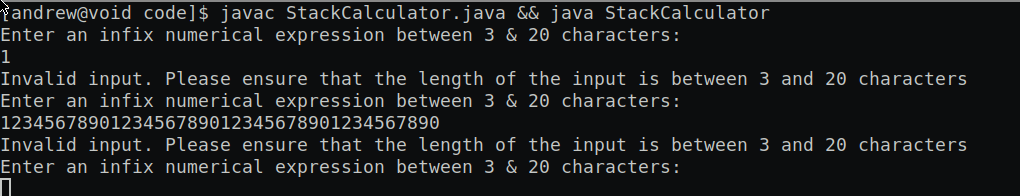
\includegraphics[width=0.7\textwidth]{images/illegallength.png}
    \caption{Testing Expressions of Illegal Length}
\end{figure}

\begin{figure}[h]
    \centering
    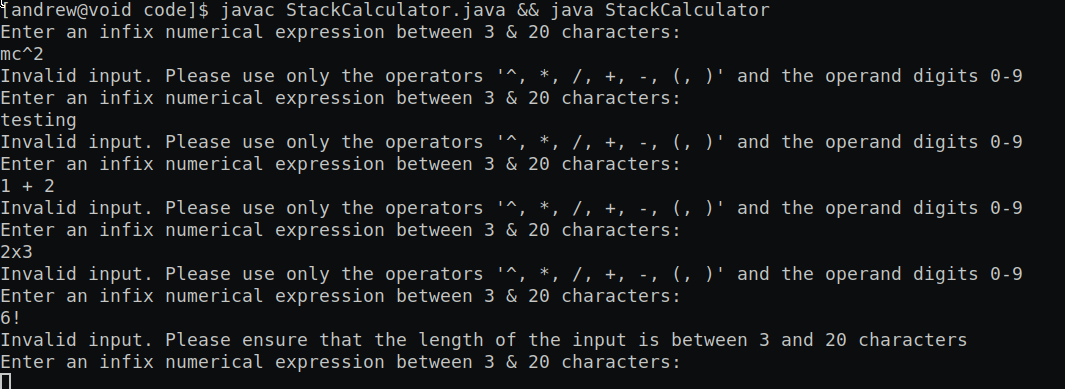
\includegraphics[width=0.7\textwidth]{images/illegalcharacters.png}
    \caption{Testing Expressions which Contain Illegal Characters}
\end{figure}

\begin{figure}[h]
    \centering
    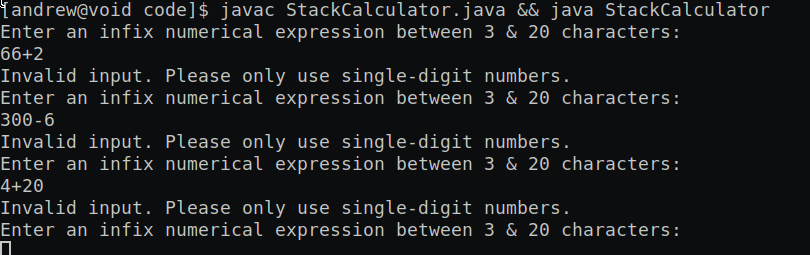
\includegraphics[width=0.7\textwidth]{images/doubledigit.png}
    \caption{Testing Expressions which Contain Double-Digit Numbers}
\end{figure}

Of course, the next thing that we must ensure is that the program accepts valid inputs. 
However, for the sake of convenience \& concision, these tests can be bundled with tests ensuring that the calculations 
work properly. 
Assuming that the program passes the tests which check if the program calculates expressions correctly, then we know 
that the program must also be accepting valid inputs.
\\\\
The next series of tests that we'll want to perform are checking that the program calculates the correct answer to the 
expressions that are entered. 
We'll want to test each operator both individually and in concert with other operators.
We expect that the program obeys the standard BIMDAS rules, and that the results match the results you would get from 
any other calculator. 

\begin{figure}[h]
    \centering
    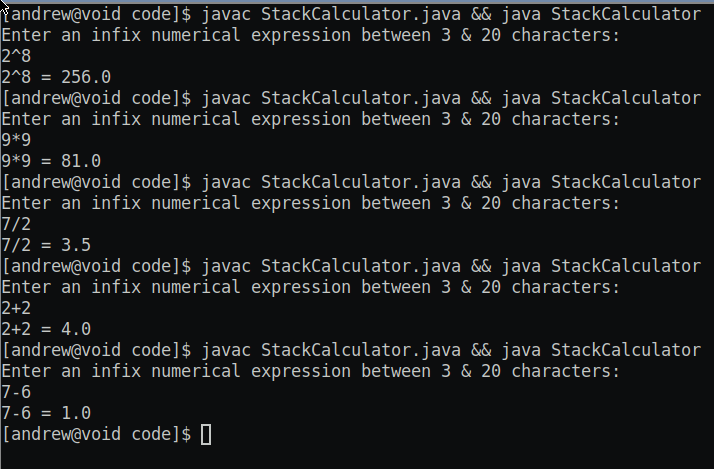
\includegraphics[width=0.7\textwidth]{images/individualoperators.png}
    \caption{Testing Each Operator Individually}
\end{figure}

\begin{figure}[h]
    \centering
    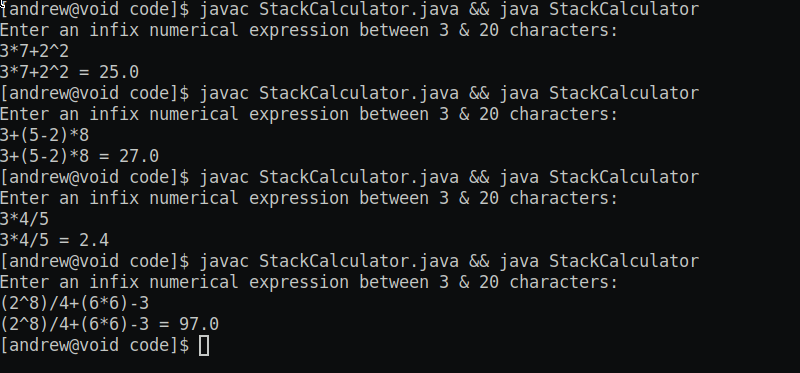
\includegraphics[width=0.7\textwidth]{images/inconcert.png}
    \caption{Testing Combinations of Operators}
\end{figure}

These screenshots demonstrate that the program behaved as expected in each potential situation. 
The program rejects invalid input, accepts valid input, and calculates the correct answer for each valid input, 
regardless of which operators or which numbers are combined together.


\end{document}
